% calculus:x08
\begin{question}
  \hspace*{\fill} [Note maximale: 15]\par
  \medskip
  \noindent La figure suivante représente une partie de la représentation graphique de la fonction quadratique $f$.\par
  \medskip
  \begin{center}
    % \noindent La figure n'est pas a l'échelle\par
    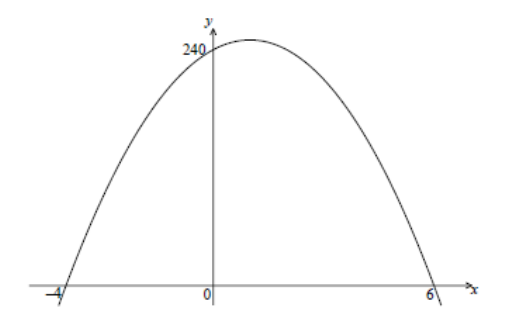
\includegraphics[scale=0.3]{temp_down_parabola}\par
  \end{center}
  \medskip
  \noindent Les abscisses à l’origine sont en (-4; 0 ) et (6; 0) et l’ordonnée à l’origine est en (0; 240).\par
  \medskip
  (a) Donnez $f(x)$ sous la forme $f(x) = -10(x - p) (x - q)$.\hspace*{\fill} [2]\par
  \medskip
  (b) Trouvez une autre expression de $f(x)$ sous la forme $f(x) = -10(x - h)^2 + k$.\hspace*{\fill} [4]\par
  \medskip
  (c) Montrez que $f(x)$ peut aussi s’écrire sous la forme $f(x) = 240 + 20x -10x^2$.\hspace*{\fill} [2]\par
  \medskip
  \noindent Une particule se déplace en ligne droite de telle sorte que sa vitesse $v$ (en $ms^{-1}$ ),
au temps $t$ (en secondes), est donnée par $v = 240 + 20t -10t^2$ , avec $0 \le t \le 6$\par
  (d)\par
  \medskip
  \hspace{1em}(i)  Trouvez la valeur de $t$ quand la vitesse de la particule est la plus grande.\par
  \hspace{1em}(ii) Trouvez l’accélération de la particule quand sa vitesse est nulle.\hspace*{\fill} [7]\par
\end{question}



